\problemname{Family Reunion}
\begin{figure}[h!]
  \centering
  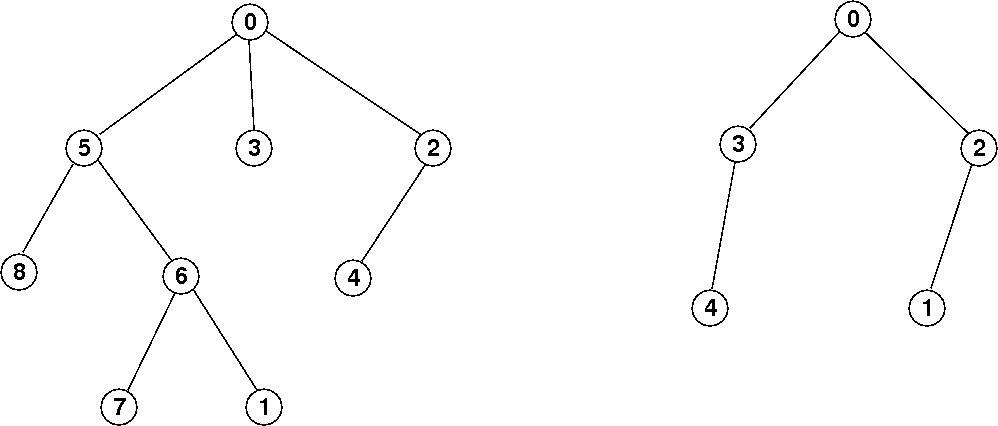
\includegraphics[width=16cm]{slakttraffen.png}
  \caption{The family trees for the two sample inputs.}
\end{figure}

It is a family reunion for the descendants of Ida-Ottilia Isaksson.
For simplicity, a family tree has been established and all descendants have been numbered from $1$ to $N$, while Ida-Ottilia herself has been given number $0$.
Among the $M$ people at your table, a discussion arises about who is your nearest common ancestor (upward in the tree).
Write a program that computes this.

The program should ask for the number of descendants, $N$, and then ask for the number of each person's parent, which is of course always between $0$ and $N$.
Then the program should ask for the number of people at the table, $M$ ($2 \le M \le N$), and read the number of each of them.
The program should output the number of the person who is the nearest common ancestor (upward in the tree) of everyone at the table.
Note that this can sometimes be someone at the table.

\section*{Input}
The first line of input contains the numbers $N$ and $M$ ($2 \le M \le N \le 20$).
The second line contains $N$ numbers, the parent of each descendant (all between $0$ and $N$).
The third line contains $M$ numbers, the people around the table (all between $1$ and $N$, without duplicates).

\section*{Output}
The program should output a single number: the number of the people's nearest common ancestor.
